% this file is called up by thesis.tex
% content in this file will be fed into the main document
\chapter{Relaciones de ortogonalidad  de los armónicos esféricos vectoriales}
% top level followed by section, subsection

\section{Apéndice}


	\begin{figure}[h!]\centering
	\begin{minipage}[c]{.95\linewidth}\centering
	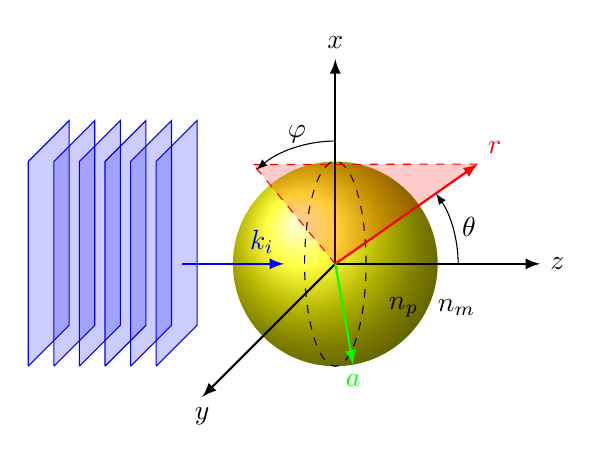
\begin{tikzpicture}[scale=1.3]

\coordinate (O) at (0,0);

%------------------------------------------------------- Particle
\shade[ball color=yellow, opacity = 1] (O) circle (1); 
\draw[dashed] (O) ellipse (.3 and 1);

%------------------------------------------------------- Coordinate system axes
\draw[- latex, thick] (O) -- (-1.3,-1.3) node[anchor=north ]{$y$};
\draw[- latex, thick] (O) -- (2,0) node[anchor= west]{$z$};
\draw[- latex, thick] (O) -- (0,2) node[anchor=south]{$x$};


%------------------------------------------------------- Vector \vb{r}
\draw[thick,red,- latex] (O) -- (35:1.7) node[anchor=south west]{$\vb{r}$}; 
\draw[-, dashed,red] (O) -- (-.8,.97);		%xy proyection
\draw[-,dashed,red] (-.8,.97) -- (35:1.7) ;	%normal proyection
\fill[red,opacity=.2] (O)-- (-.8,.97)--(35:1.7)--(O);  %Shade
	
	
%------------------------------------------------------- polar variables	
\path (O)++(35/2:1.2)node[anchor=west]{$\theta$};    
\draw[- latex](0:1.2)arc(0:35:1.2);

\path (O)++(100:1.1)node[anchor=south east]{$\varphi$};    
\draw[- latex](90:1.2)arc(90:130:1.2);
	

%------------------------------------------------------- Particule radius & n	
\draw[thick,green,- latex] (O) -- (-80:1) node[anchor=north]{$\vb{a}$};  

\path (O)++(-25:1) node[anchor=east]{$n_p$};
\path (O)++(-25:1) node[anchor=west]{$n_m$};


%------------------------------------------------------- Plane wave

\def\dx{1.75}
\def\dy{1}
\def\dr{.4}

\foreach \i in {-5,...,-1,0}{
	\fill[opacity=.2,blue] (\i*.25-\dx,-\dy)--(\i*.25-\dx,\dy)--
							(\i*.25-\dx+\dr, \dy+\dr)--(\i*.25-\dx+\dr, -\dy+\dr);
	\draw[blue] (\i*.25-\dx,-\dy)--(\i*.25-\dx,\dy)--
							(\i*.25-\dx+\dr, \dy+\dr)--(\i*.25-\dx+\dr, -\dy+\dr)--
							(\i*.25-\dx,-\dy);}									

\draw[- latex,thick,blue] (-1.5,0)--(-1.5+1,0) node[anchor=south east]{$\vb{k}_i$};

	
\end{tikzpicture}
		\caption{ Esfera de radio $a$ e ínidce de refracción $n_p$, inmersa en una matriz con índice $n_m$. La esfera es iluminada por una onda plana de luz con vector de onda $\vb{k}_i$ que viaja en la dirección $\hat{e}_z$.}\label{fig:EsferaA}
	\end{minipage}
	\end{figure}

Los armónicos esféricos vectoriales son solución a la ecuación de Helmholtz, por lo que cualquier solución de campo EM puede escribirse como una serie infinta en términos de las Ecs. \eqref{eq:AEV}. Para resolver el problema de los campos EMs esparcidos por una partícula esférica, se expande una onda plana $\vb{E}^i$ en la base de los armónicos esféricos vectoriales. Para esto, se emplean sus  condiciones de ortogonalidad.

Las funciones $\sin(m\varphi)$ y $\cos(m\varphi)$ obedecen las relaciones de ortogonalidad
 	\begin{subequations}
	\begin{align}
	\int_0^{2\pi} \sin(m\varphi) &\cos(m' \varphi) \dd\varphi = 0 \qquad \forall\, m,m',\label{seq:ortSinCos}\\
	\int_0^{2\pi} \sin(m\varphi) \sin(m'\varphi)\dd\varphi &=  \int_0^{2\pi} \cos(m\varphi) \cos(m'\varphi)\dd\varphi  = \delta_{m,m'}\frac{\pi}{2}.\label{seq:ortCos2}
	\end{align}\label{eq:SinCos}
 	\end{subequations}
Por la Ec. \eqref{seq:ortSinCos} se cumple que el producto interior\footnote{Se define el producto interior $\langle \vb{A},\vb{B} \rangle_{\theta,\varphi}$ como $\langle \vb{A},\vb{B} \rangle_{\theta,\varphi} \equiv \int_0^{2\pi}\int_0^\pi \vb{A}\cdot\vb{B} \sin\theta \dd\theta \dd\varphi$} entre $\vb{M}_{em\ell}$ y $\vb{M}_{om'\ell'}$, y $\vb{N}_{em\ell}$ y $\vb{N}_{om'\ell'}$ es
	\begin{tcolorbox}[ ams align ]
		\langle\vb{M}_{em\ell}, \vb{M}_{om'\ell'} \rangle_{\theta,\varphi} =
		\langle\vb{N}_{em\ell}, \vb{N}_{om'\ell'} \rangle_{\theta,\varphi} = 0
		&\qquad \forall\,  m,m',\ell, \ell',\\
		\intertext{así como también}
		\langle\vb{M}_{om\ell}, \vb{N}_{em'\ell'} \rangle_{\theta,\varphi} = 
		\langle\vb{M}_{om\ell}, \vb{N}_{om'\ell'} \rangle_{\theta,\varphi} = 	
		\langle\vb{M}_{em\ell}, \vb{N}_{em'\ell'} \rangle_{\theta,\varphi} = 	0
		&\qquad \forall\,  m,m',\ell, \ell'.				
	\end{tcolorbox}\noindent
pues $\vb{M}$ tiene componente nula en $\vu{e}_r$ y en los demás términos se encuentra la Ec. \eqref{seq:ortSinCos}. Las Ecs. \eqref{eq:SinCos} implican que todos los armónicos esféricos vectoriales orden $m$ distinto  son ortogonales entre sí.\\

 El producto interior entre $\vb{M}_{em\ell}$ y $\vb{N}_{om\ell'}$, empleando el resultado de la Ec. \eqref{seq:ortCos2} con $m=m'$, está dado por
	\begin{align}
		\langle\vb{M}_{em\ell},  \vb{N}_{om\ell'} \rangle_{\theta,\varphi} &= - \frac{\pi}{2} \frac{z_\ell (\rho)}{\rho}\dv{z_{\ell'}(\rho)}{\rho}	m
							 \int_0^\pi\qty[P_\ell^m(\cos \theta )\dv{P_{\ell'}^m(\cos \theta )}{\theta}+ 
							  \dv{P_{\ell}^m(\cos \theta )}{\theta}P_{\ell'}^m(\cos \theta )] \dd\theta \notag\\
					 &=- \frac{\pi}{2} \frac{z_\ell (\rho)}{\rho}\dv{z_{\ell'}(\rho)}{\rho}	m 
					 	\int_0^\pi \dv{\theta}\qty[P_\ell^m(\cos\theta)P_{\ell'}^m(\cos\theta)]\dd\theta \notag\\
					 &=- \frac{\pi}{2} \frac{z_\ell (\rho)}{\rho}\dv{z_{\ell'}(\rho)}{\rho}	m \eval{P_\ell^m(\cos\theta)P_{\ell'}^m(\cos\theta)}_0^\pi.
					 	\label{eq:MeNo}
	\end{align}
Mediante un procedimiento semejante se obtiene que $\langle\vb{M}_{em\ell},  \vb{N}_{om\ell'} \rangle_{\theta,\varphi}=\langle\vb{M}_{om\ell},  \vb{N}_{em\ell'} \rangle_{\theta,\varphi}$. Haciendo uso de la relación entre las funciones asociadas de Legndre con los polinomios de Legendre [Ec. \eqref{eq:FAL-PL}] se obtiene que $P_\ell^m(\cos\theta)=0$ para $\theta=0,\pi$ y $m\neq 0$. Sin embargo, si en la Ec. \eqref{eq:MeNo} $m$ es igual a cero, el producto interior también es nulo, por lo que se cumple que 
	\begin{tcolorbox}[ ams align ]
		\langle\vb{M}_{em\ell},  \vb{N}_{om\ell'} \rangle_{\theta,\varphi}=
		\langle\vb{M}_{om\ell},  \vb{N}_{em\ell'} \rangle_{\theta,\varphi}= 0	
		\qquad \forall\, \ell, \ell'\, m.
	\end{tcolorbox}
Las expresiones del  producto interior entre $\vb{M}_{em\ell}$ y $\vb{M}_{em\ell'}$, y $\vb{N}_{em\ell}$ y $\vb{N}_{em\ell'}$, empleando el resultado de la Ec. \eqref{seq:ortCos2} con $m=m'$, y la relación de ortogonalidad de las funciones asociadas de Legendre [Ec. \eqref{eq:ortLegendre}] son
	\begin{align*}
		\langle\vb{M}_{em\ell},  \vb{M}_{em\ell'} \rangle_{\theta,\varphi} =& 
				\frac{\pi}{2} z_\ell (\rho) z_{\ell'}(\rho)\times	 \int_0^\pi\qty[\frac{m^2}{\sin^2\theta}P_\ell^m(\cos\theta)P_{\ell'}^m(\cos\theta)
				 +\dv{P_\ell^m(\cos\theta)}{\theta}\dv{P_{\ell'}^m(\cos\theta)}{\theta}]\sin\theta\dd\theta\\
		\langle\vb{N}_{em\ell},  \vb{N}_{em\ell'} \rangle_{\theta,\varphi} =&
				\frac{\pi}{2} \qty[\frac{z_\ell(\rho)}{\rho}\ell(\ell+1)]^2\frac{2}{2\ell+1}\frac{(\ell+m)!}{(\ell-m)!}\delta_\ell^{\ell'}+
				\frac{\pi}{2} \frac{1}{\rho^2}\dv{\rho}\qty[\rho z_\ell (\rho)]\dv{\rho}\qty[\rho z_{\ell'}(\rho)]\\
				&\times \int_0^\pi\qty[\frac{m^2}{\sin^2\theta}P_\ell^m(\cos\theta)P_{\ell'}^m(\cos\theta)
					+\dv{P_\ell^m(\cos\theta)}{\theta}\dv{P_{\ell'}^m(\cos\theta)}{\theta}]\sin\theta\dd\theta.				 
	\end{align*}
Asimismo, se cumple que  $\langle\vb{M}_{em\ell},  \vb{M}_{em\ell'} \rangle_{\theta,\varphi}=\langle\vb{M}_{om\ell},  \vb{M}_{om\ell'} \rangle_{\theta,\varphi}$ y $\langle\vb{N}_{em\ell},  \vb{N}_{em\ell'} \rangle_{\theta,\varphi}=\langle\vb{N}_{om\ell},  \vb{N}_{om\ell'} \rangle_{\theta,\varphi}$. Sustituyendo $P_\ell^m(\cos\theta)$ en la Ec. \eqref{eq:Theta} y multiplicándola por $P_{\ell'}^m(\cos\theta)$, operando de la misma forma intercambiando los papeles de $P_\ell^m(\cos\theta)$  y $P_{\ell'}^m(\cos\theta)$ y sumando ambos resultados se llega a la expresión 
	\begin{align}
	2\frac{m^2}{\sin^2\theta}P_\ell^m P_{\ell'}^m \sin\theta =&
					 P_\ell\dv{\theta}\qty[\sin\theta \dv{P_{\ell'}^m}{\theta}] P_{\ell'}\dv{\theta}\qty[\sin\theta \dv{P_\ell^m}{\theta}]
					 +	\ell(\ell+1)P_\ell^m P_{\ell'}^m	 \sin\theta  \notag\\
					 &+ \ell'(\ell'+1)P_\ell^m P_{\ell'}^m\sin\theta, \label{eq:PnPn'}
	\end{align}
en donde se obvia el argumento $\cos\theta$. Dado que 
	\begin{equation*}
	\dv{\theta}\qty[P_{\ell'}^m\sin\theta  \dv{P_\ell^m}{\theta}] 
	= P_{\ell'}^m\dv{\theta}\qty[\sin\theta \dv{P_\ell^m}{\theta}] + \sin\theta\dv{P_{\ell'}^m}{\theta}\dv{P_\ell^m}{\theta},
	\end{equation*}
sumando $2\sin\theta\dd P_{\ell'}^m\dd\theta \dd P_\ell^m \dd\theta$ de ambos lados de la Ec. \eqref{eq:PnPn'} y agrupando términos, se obtiene que el integrando presente en los productos interiores de  $\vb{M}_{em\ell}$ y $\vb{M}_{em\ell'}$, y $\vb{N}_{em\ell}$ y $\vb{N}_{em\ell'}$ es
	\begin{align*}
	\qty[\frac{m^2}{\sin^2\theta}P_\ell^mP_{\ell'}^m	+\dv{P_\ell^m}{\theta}\dv{P_{\ell'}^m}{\theta}]\sin\theta = &
					 \frac12 \dv{\theta}\qty[\sin\theta \dv{P_{\ell'}^m}{\theta}P_\ell^m + \sin\theta\dv{P_{\ell}^m}{\theta}P_{\ell'}^m ]
					 +	\frac12 \ell(\ell+1)P_\ell^m P_{\ell'}^m	 \sin\theta  \\
					 &+ \frac12 \ell'(\ell'+1)P_\ell^m P_{\ell'}^m\sin\theta,
	\end{align*}
en donde el primer término de la suma se desvanece al evaluarse en $\theta=0,\pi$ y los últimos cumplen con la relación de ortogonalidad de la Ec. \eqref{eq:ortLegendre}. Por lo tanto
	\begin{tcolorbox}[ ams align ]
		\langle\vb{M}_{em\ell},  \vb{M}_{em\ell'} \rangle_{\theta,\varphi}=&	\langle\vb{M}_{om\ell},  \vb{M}_{om\ell'} \rangle_{\theta,\varphi} 
										=\delta_\ell^{\ell'}\pi z_\ell (\rho)^2\frac{\ell(\ell+1)}{2\ell+1}\frac{(\ell+m)!}{(\ell-m)!}
		&\quad \forall\, \ell, \ell',\, m, \label{eq:MM} \\
		\langle\vb{N}_{em\ell},  \vb{N}_{em\ell'} \rangle_{\theta,\varphi}=&	\langle\vb{N}_{om\ell},  \vb{N}_{om\ell'} \rangle_{\theta,\varphi} \notag\\
										=&\delta_\ell^{\ell'}\pi\frac{\ell(\ell+1)}{2\ell+1}\frac{(\ell+m)!}{(\ell-m)!}\left\{ \qty[\frac{z_\ell(\rho)}{\rho}]^2 \ell(\ell+1)+
										   \qty[\frac{1}{\rho}\dv{[\rho z_\ell (\rho)]}{\rho}]^2  \right\}
		&\quad \forall\, \ell, \ell',\, m.	\label{eq:NN}
	\end{tcolorbox}
